\documentclass{standalone}
\usepackage[utf8]{inputenc}
\usepackage{amsmath}
\usepackage{amsfonts}
\usepackage{amssymb}
\usepackage{tikz}
\usetikzlibrary{calc}

% GanttHeader setups some parameters for the rest of the diagram
% #1 Width of the diagram
% #2 Width of the space reserved for task numbers
% #3 Width of the space reserved for task names
% #4 Number of months in the diagram
% In addition to these parameters, the layout of the diagram is influenced
% by keys defined below, such as y, which changes the vertical scale
\def\GanttHeader#1#2#3#4{%
 \pgfmathparse{(#1-#2-#3)/(#4)}
 \tikzset{y=7mm, task number/.style={left, font=\bfseries},
     task description/.style={text width=#3,  right, draw=none,
           font=\sffamily, xshift=#2,
           minimum height=2em},
     gantt bar/.style={draw=black, fill=blue!30},
     help lines/.style={draw=black!30, dashed},
     x=\pgfmathresult pt
     }
  \def\totalmonths{#4}
  \node (Header) [task description] at (0,0) {\textbf{\large }};
  \begin{scope}[shift=($(Header.south east)$)]
    \foreach \x in {1,...,#4}
      \node[above,rotate=90] at (\x,1) {\tiny\x};
 \end{scope}
}

% This macro adds a task to the diagram
% #1 Number of the task
% #2 Task's name
% #3 Starting date of the task (month's number, can be non-integer)
% #4 Task's duration in months (can be non-integer)
\def\Task#1#2{%
%\node[task number] at ($(Header.west) + (0, -#1)$) {#1};
\node[task description] at (0,-#1) {#2};
\begin{scope}[shift=($(Header.south east)$)]
  \draw (0,-#1) rectangle +(\totalmonths, 1);
  \foreach \x in {1,...,\totalmonths}
    \draw[help lines] (\x,-#1) -- +(0,1);
\end{scope}
}

% This macro adds a task to the diagram
% #1 Number of the task
% #2 Task's name
% #3 Starting date of the task (month's number, can be non-integer)
% #4 Task's duration in months (can be non-integer)
\def\TaskActive#1#2#3{%
\begin{scope}[shift=($(Header.south east)$)]
  \filldraw[gantt bar] ($(#2, -#1+0.2)$) rectangle +(#3,0.6);
\end{scope}
}

\begin{document}

\begin{tabular}{l}
\begin{tabular}{lr}
Scheduler: & RR-3 scheduler
\\
Input: & input/testdata3.txt
\\
Total Process Count: & 17
\\
Total Waiting Time: & 2055
\\
Average Waiting Time: & 120.882355
\\
Total Turnaround Time: & 2259
\\
Average Turnaround Time: & 132.88235
\\
Total Context Switch Count: & 73
\\
\end{tabular}
\\
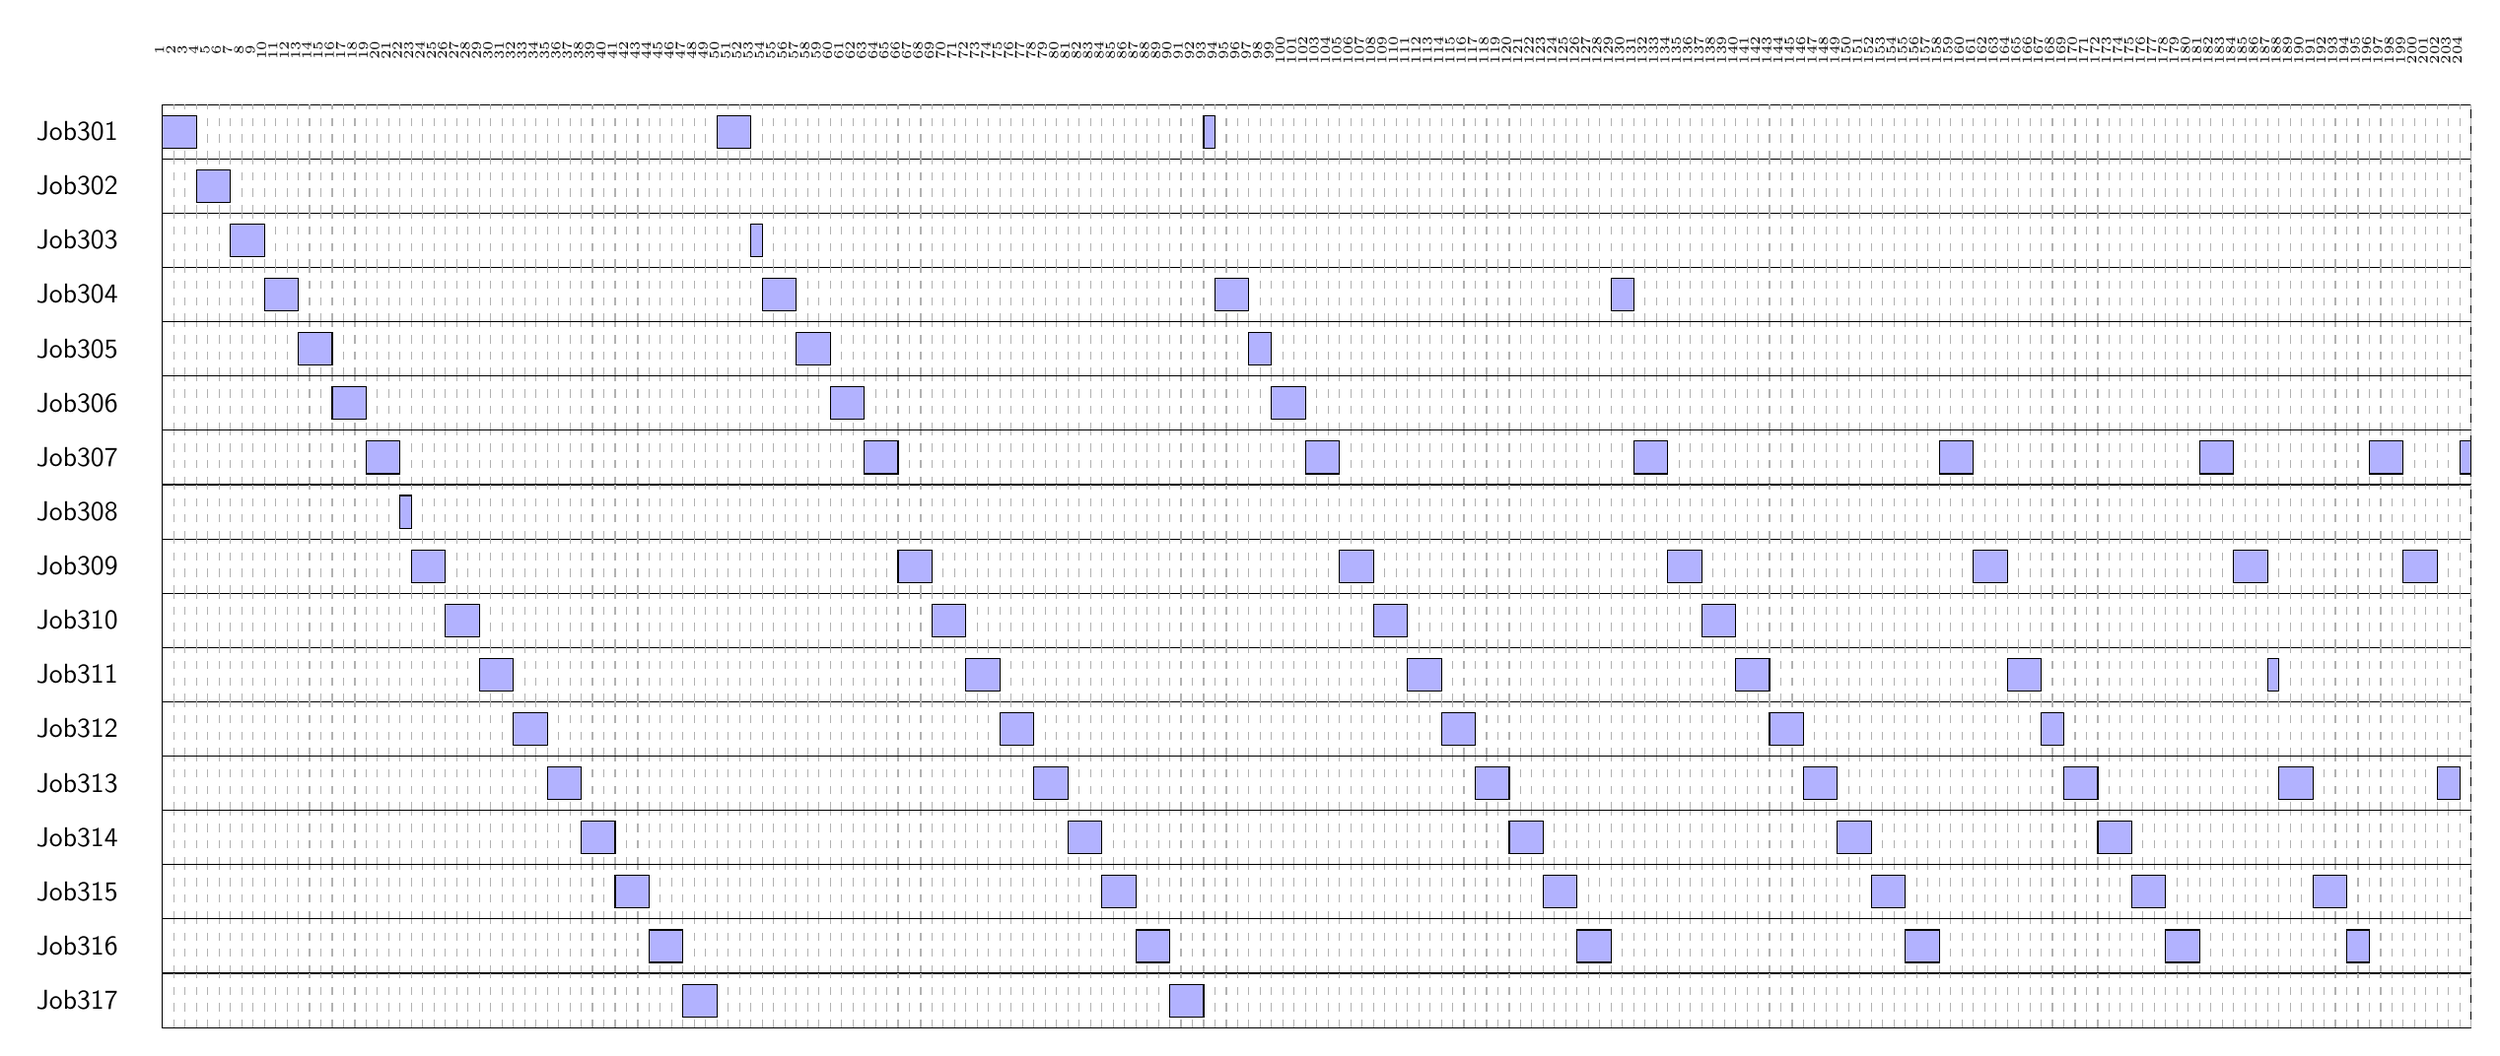
\begin{tikzpicture}
\GanttHeader{32cm}{5ex}{1.5cm}{204}
\Task{1}{Job301}
\Task{2}{Job302}
\Task{3}{Job303}
\Task{4}{Job304}
\Task{5}{Job305}
\Task{6}{Job306}
\Task{7}{Job307}
\Task{8}{Job308}
\Task{9}{Job309}
\Task{10}{Job310}
\Task{11}{Job311}
\Task{12}{Job312}
\Task{13}{Job313}
\Task{14}{Job314}
\Task{15}{Job315}
\Task{16}{Job316}
\Task{17}{Job317}
\TaskActive{1}{0}{3}
\TaskActive{2}{3}{3}
\TaskActive{3}{6}{3}
\TaskActive{4}{9}{3}
\TaskActive{5}{12}{3}
\TaskActive{6}{15}{3}
\TaskActive{7}{18}{3}
\TaskActive{8}{21}{1}
\TaskActive{9}{22}{3}
\TaskActive{10}{25}{3}
\TaskActive{11}{28}{3}
\TaskActive{12}{31}{3}
\TaskActive{13}{34}{3}
\TaskActive{14}{37}{3}
\TaskActive{15}{40}{3}
\TaskActive{16}{43}{3}
\TaskActive{17}{46}{3}
\TaskActive{1}{49}{3}
\TaskActive{3}{52}{1}
\TaskActive{4}{53}{3}
\TaskActive{5}{56}{3}
\TaskActive{6}{59}{3}
\TaskActive{7}{62}{3}
\TaskActive{9}{65}{3}
\TaskActive{10}{68}{3}
\TaskActive{11}{71}{3}
\TaskActive{12}{74}{3}
\TaskActive{13}{77}{3}
\TaskActive{14}{80}{3}
\TaskActive{15}{83}{3}
\TaskActive{16}{86}{3}
\TaskActive{17}{89}{3}
\TaskActive{1}{92}{1}
\TaskActive{4}{93}{3}
\TaskActive{5}{96}{2}
\TaskActive{6}{98}{3}
\TaskActive{7}{101}{3}
\TaskActive{9}{104}{3}
\TaskActive{10}{107}{3}
\TaskActive{11}{110}{3}
\TaskActive{12}{113}{3}
\TaskActive{13}{116}{3}
\TaskActive{14}{119}{3}
\TaskActive{15}{122}{3}
\TaskActive{16}{125}{3}
\TaskActive{4}{128}{2}
\TaskActive{7}{130}{3}
\TaskActive{9}{133}{3}
\TaskActive{10}{136}{3}
\TaskActive{11}{139}{3}
\TaskActive{12}{142}{3}
\TaskActive{13}{145}{3}
\TaskActive{14}{148}{3}
\TaskActive{15}{151}{3}
\TaskActive{16}{154}{3}
\TaskActive{7}{157}{3}
\TaskActive{9}{160}{3}
\TaskActive{11}{163}{3}
\TaskActive{12}{166}{2}
\TaskActive{13}{168}{3}
\TaskActive{14}{171}{3}
\TaskActive{15}{174}{3}
\TaskActive{16}{177}{3}
\TaskActive{7}{180}{3}
\TaskActive{9}{183}{3}
\TaskActive{11}{186}{1}
\TaskActive{13}{187}{3}
\TaskActive{15}{190}{3}
\TaskActive{16}{193}{2}
\TaskActive{7}{195}{3}
\TaskActive{9}{198}{3}
\TaskActive{13}{201}{2}
\TaskActive{7}{203}{1}
\end{tikzpicture}
\end{tabular}
\end{document}
